\documentclass[UKenglish,aspectratio=169]{beamer}
\usepackage[utf8]{inputenc}
\usepackage{babel, textcomp}
% \usepackage{arevtext}
\usepackage{microtype}
\usepackage{appendixnumberbeamer}
\usepackage{graphicx}

\usepackage{tikz}
\usepackage{tikz-cd}
\usetikzlibrary{calc}
\usetikzlibrary{intersections}
\usetikzlibrary{decorations.markings}

\usepackage{amsmath, amssymb}

\usepackage{hyperref}
\usepackage{xcolor}
\setbeamertemplate{caption}[numbered]
% \hypersetup{ % this is just my personal choice, feel free to change things
%     % colorlinks,
%     % linkcolor={red!50!black},
%     citecolor={blue!50!black},
%     urlcolor={blue!80!black},
% }

\usetheme[
    uiostandard,
    toc,
    font=arial,
    sectionsep=uiogreen2,
]{UiO}
\usefonttheme{professionalfonts}
\usefonttheme[onlymath]{serif}
\urlstyle{sf}

\title{Configurations of lines in surfaces}
\author{Mikkel Gjestrud}

\begin{document}
\uiofrontpage[
    % info={A minimal user guide},
    % image={uio-beamer-segl-pos},
    date={12th December, 2025},
]

\begin{frame}{Conventions}
    \begin{itemize}
        % \item $\Bbbk$ denotes an algebraically closed field of characteristic $0$.
        \item We work over the field of complex numbers $\mathbb{C}$.
        % \item $K(X)$ denotes the function field of a variety $X$.
        % \item $K(X)^\times$ denotes the multiplicative group of non-zero elements in $K(X)$.
        \item We denote $\dim_\mathbb{C} H^i(-,-)$ by $h^i(-,-)$.
        \item We work in $\mathbb{P}^3$ with homogeneous coordinates $(x_0 : x_1 : x_2 : x_3)$.
    \end{itemize}
\end{frame}

\begin{frame}{Motivation}
    \begin{itemize}
        \item 27 lines on a smooth cubic surface.
        \item Eckardt points on cubic surfaces.
        \item Which configurations do we `expect' to find in surfaces of degree $d$?
        \item When can we find a surface of degree $d$ including a given configuration of lines? And is it smooth?
        % \item Lines in surfaces is a classical topic in algebraic geometry.
        % \item The famous result that a smooth cubic surface contains exactly 27 lines.
        % \item What configurations of lines can we find in surfaces of degree $d$?
        % \item When can we find smooth surfaces including given configurations of lines?
    \end{itemize}
\end{frame}

\begin{frame}{Cayley-Salmon theorem}
    \begin{theorem}
        A smooth cubic surface $S_3 \subseteq \mathbb{P}^3$ contains exactly 27 lines.
    \end{theorem}
    % \begin{figure}
    %     \centering
    %     \input{../doc/figures/27lines.tex}
    % \caption{Clebsch surface.}
    % \end{figure}
    
\end{frame}

\begin{frame}[fragile]{Blow-up of $\mathbb{P}^2$ in six points}
    \begin{figure}
        \centering
        % Improved schematic of the blow-up of $\mathbb{P}^2$ in six points.
% Shows six points in general position and highlights the strict transform of the line $\ell_{25}$.
% The other 14 lines through pairs are omitted to keep the figure uncluttered.
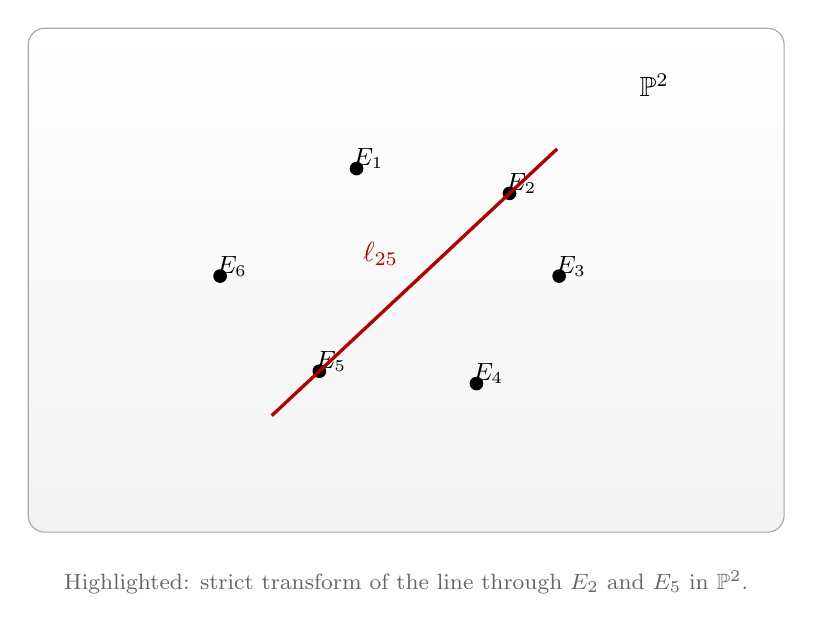
\begin{tikzpicture}[scale=1.05,
	plane/.style = {draw=black!35, top color=white, bottom color=black!5, rounded corners=6pt, minimum width=9.6cm, minimum height=6.4cm},
	pt/.style = {draw=black, fill=white, circle, inner sep=1.9pt, line width=0.5pt},
	blowpt/.style = {draw=black, fill=black, circle, inner sep=1.6pt},
	linebase/.style = {line width=0.9pt, color=black!35},
	selline/.style = {line width=1.2pt, color=red!70!black},
	lab/.style = {font=\small, inner sep=1pt}
]

% Subtle background representing $\mathbb{P}^2$ before blow-up
\node[plane] (P2) at (0,0) {};
\node[lab, font=\normalsize] at ($(P2.north)+(3.0cm,-7mm)$) {$\mathbb{P}^2$};

% Six points in general position (now labeled $E_1,\dots,E_6$ to emphasize exceptional curves)
\coordinate (E1) at ($(P2.center)+(-0.6,1.35)$);
\coordinate (E2) at ($(P2.center)+(1.25,1.05)$);
\coordinate (E3) at ($(P2.center)+(1.85,0.05)$);
\coordinate (E4) at ($(P2.center)+(0.85,-1.25)$);
\coordinate (E5) at ($(P2.center)+(-1.05,-1.10)$);
\coordinate (E6) at ($(P2.center)+(-2.25,0.05)$);

% Draw the six marked points representing exceptional curves $E_i$
\foreach \Q/\LBL in {E1/$E_1$, E2/$E_2$, E3/$E_3$, E4/$E_4$, E5/$E_5$, E6/$E_6$} {
  \node[blowpt] at (\Q) {};
  \node[lab] at ($(\Q)+(0.14,0.12)$) {\LBL};
}

% Highlight ONE line: strict transform of the line passing through the two centers giving $E_2$ and $E_5$.
% We extend it slightly to suggest the original line in $\mathbb{P}^2$.
\path let \p1 = (E2), \p2 = (E5) in
  coordinate (ExtA) at ($(E2)!1.25!(E5)$)
  coordinate (ExtB) at ($(E2)!-0.25!(E5)$);
\draw[selline] (ExtA) -- (ExtB) node[midway, above left=2pt] {$\ell_{25}$};

% (Optional) Previously showed gray circles to hint exceptional divisors; removed for consistency since points now labeled $E_i$.

% Optional very faint hints of a few other pair-lines (commented out to keep clarity)
% \draw[linebase,dashed] ($(P1)!1.15!(P2pt)$) -- ($(P1)!-0.15!(P2pt)$);
% \draw[linebase,dashed] ($(P3)!1.10!(P4)$) -- ($(P3)!-0.10!(P4)$);
% \draw[linebase,dashed] ($(P6)!1.10!(P1)$) -- ($(P6)!-0.10!(P1)$);

% Annotation at bottom explaining conventions
\node[font=\footnotesize, align=center, color=black!60] at ($(P2.south)+(0,-6mm)$) {Highlighted: strict transform of the line through $E_2$ and $E_5$ in $\mathbb{P}^2$.};

\end{tikzpicture}
    % \caption{A 4-chain in $\mathbb{P}^3$.}
    \end{figure}
\end{frame}


\begin{frame}{$m$-cross}
    \begin{figure}
        \centering
        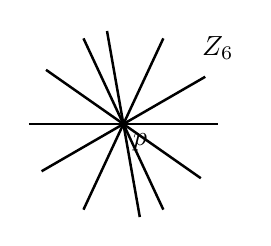
\begin{tikzpicture}[scale=0.4]
% Six lines passing through a common point p at the origin
% Draw the six lines without inline labels
\foreach \theta in {115,-80,65,-35,30,0} {
    \draw[rotate=\theta, line width=0.9pt] (-3,0) -- (3,0);
}
% Common intersection point p
\fill (0,0) circle (2pt) node[below right] {$p$};

% Optional label
\node at (3,2.4) {$Z_6$};
\end{tikzpicture}
    \caption{A 6-cross in $\mathbb{P}^3$.}
    \label{fig:Z_6}
    \end{figure}
    \begin{definition}
        An $m$-cross is a union of $m$ distinct lines $l_1, l_2, \dots, l_m$ in $\mathbb{P}^3$ which intersect at a common point $p$ and lying in a common plane $H$. We will write $Z_m = \bigcup_{i=1}^m l_i$.
    \end{definition}
\end{frame}

\begin{frame}
        \begin{theorem}
        Given an $m$-cross, we can find a smooth surface $S_d$ of degree $d$ including it if and only if $d = 1$ or $d \geq m$.
    \end{theorem}

    Key idea: Automorphism of $\mathbb{P}^3$ gives
    % can be used to move an $m$-cross into a position where we can construct such a surface. Explicitly, we move the lines to 
    \[l_1 = (\alpha : \beta : 0 : 0), \ l_2 = (\alpha : 0 : \gamma : 0), \ l_3=(\alpha: \lambda_3 \delta : \delta: 0), \dots, l_m = (\alpha :\lambda_m  \delta : \delta : 0)\]

    These lines all intersect at the point $p = (1 : 0 : 0 : 0)$ and lie in the plane $H = V(x_3)$.
\end{frame}

\begin{frame}
    \begin{figure}
        \centering
        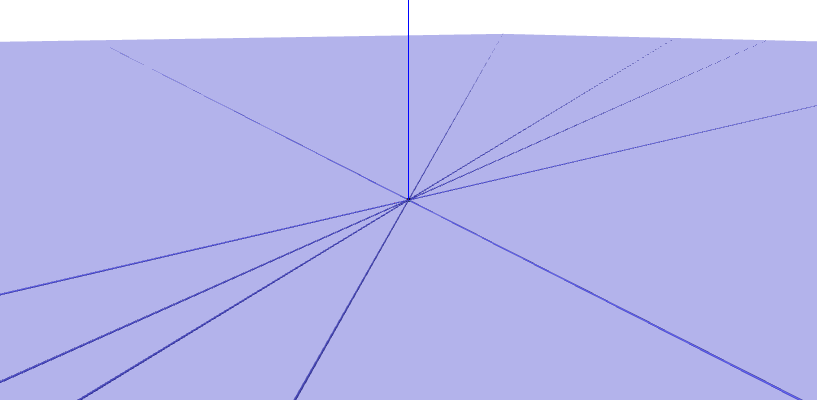
\includegraphics[width=0.8\textwidth]{../doc/figures/plane.png}
    \caption{A 5-cross in a plane $H$ in the affine patch $x_0 = 1$.}
    \end{figure}
\end{frame}

\begin{frame}
    \begin{itemize}
        \item If $d=1$, we can take $X = H$.
        \item If $1 < d < m$, no such surface exists by Bezout's theorem. 
        % Consider a surface $X \subset \mathbb{P}^3$ of degree $d$ containing an $m$-cross $Z_m$, and a line in $H$ not passing through $p$. We use Bezout's theorem to see that this line must intersect $X$ in at least $d$ points, and since it intersects each line, we must have $d \geq m$ when $X$ is not equal to $H$.
        \item If $d \geq m$, we can prove that there exists such a surface. 
        % We consider a linear system with base locus $Z_m$, and find a surface which is smooth on $Z_m$. Then we apply Bertini's theorem to see that a general member of the linear system is smooth away from $Z_m$. Then we can find a surface of degree $m$ containing $Z_m$.
    \end{itemize}

    The linear system
    \[\mathfrak{L} = \{X \mid Z_m \subseteq X\}\]
    has base locus $Z_m$. We look for a surface in $\mathfrak{L}$ which is smooth on $Z_m$.

    The lines are described by 
    \[l_1 = V(x_3, x_2), \ l_2 = V(x_3, x_1), \ l_3 = V(x_3, x_1 - \lambda_3 x_2), \ \dots, \ l_m = V(x_3, x_1 - \lambda_m x_2).\]
    Define the function
    \[f(x_0, x_1, x_2, x_3) = x_1x_2 \prod_{i=3}^m (x_1 - \lambda_i x_2) + x_0^{m-1}x_3.\]

    Can show that $f$ is smooth on $Z_m$, and apply Bertini's theorem to get a smooth surface in $\mathfrak{L}$.
\end{frame}

\begin{frame}
    \begin{figure}
        \centering
        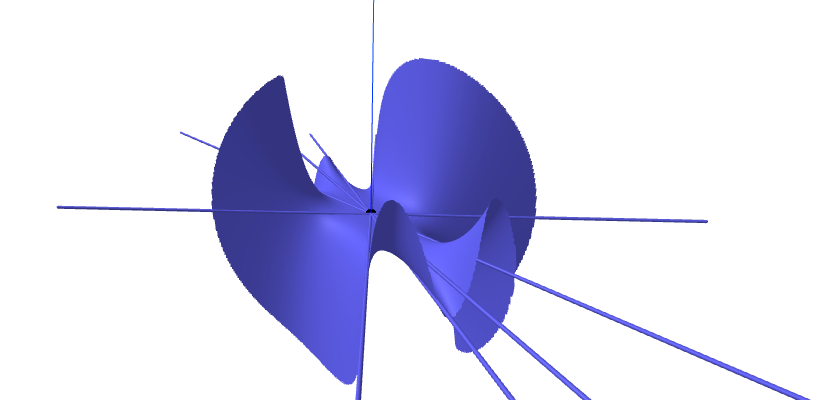
\includegraphics[width=0.9\textwidth]{../doc/figures/5cross.png}
    \caption{A 5-cross with $f$ in affine patch $x_0 = 1$.}
    \end{figure}
\end{frame}

\begin{frame}
    \begin{theorem}
        Let $A_m = \{S_d \subseteq \mathbb{P}^3 \mid Z_m \subset S_d\}$ be the set of degree $d$ surfaces containing a general $Z_m$. Then $\dim{A_m} = \binom{d-m+2}{2} + \binom{d+2}{3} - 1$ when $d \geq m$.
    \end{theorem}
\end{frame}

\begin{frame}[fragile]{$m$-gon}
    \begin{definition}
        An $m$-gon is a union of $m$ lines $l_1, l_2, \dots, l_m$ such that $l_i$ intersects $l_{i+1}$ for $1 \leq i < m$, and $l_m$ intersects $l_1$. We will write $C_m = \bigcup_{i=1}^m l_i$ and denote the intersection points as $p_i = l_i \cap l_{i+1}$ for $1 \leq i < m$, and $p_m = l_m \cap l_1$.
    \end{definition}
    We say that an $m$-gon is \emph{regular} if it only intersects at the points $p_1, p_2, \dots, p_m$, and there are no double lines. 

    Include figure.
    % \begin{figure}
    %     \centering
    %     % define a macro that draws a m-gon placed on a circle
\newcommand{\mgon}[1]{%
    \begin{tikzpicture}[scale=1, every node/.style={font=\small}]
        % radius of circle
        \def\R{2.2cm}
        \pgfmathparse{int(#1)}\let\K\pgfmathresult
        % place the points on a circle and draw the lines
        \foreach \i in {1,...,\K} {
            \pgfmathsetmacro{\ang}{90 - 360*(\i-1)/\K}
            \coordinate (P\i) at (\ang:\R);
        }
        % draw the edges (lines) and label them l_i at the midpoint
        \foreach \i in {1,...,\K} {
            \pgfmathtruncatemacro{\j}{ifthenelse(\i==\K,1,\i+1)}
            \draw[line width=0.9pt] (P\i) -- (P\j) node[midway, above, font=\small] {$l_{\i}$};
        }
        % draw and label intersection points p_i (small filled dots)
        \foreach \i in {1,...,\K} {
            \fill (P\i) circle (2.4pt) node[below right=1mm and 1mm] {$p_{\i}$};
        }
    \end{tikzpicture}
}

% Example: draw a 7-gon (change the number to any m you want)
\mgon{7}
    %     \caption{7-gon drawn in a plane.}
    %     \label{fig:m-gon}
    % \end{figure}
\end{frame}


\begin{frame}[fragile]
        \begin{theorem}
        Given a regular $m$-gon, we can find a smooth surface $S_d$ of degree $d$ including it when $m < \binom{d+3}{3}\cdot \frac{1}{d}$.
    \end{theorem}
    
    Observe this with the sequence:
    \[0 \to \mathcal{I}_{C_m}(d) \to \mathcal{O}_{\mathbb{P}^3}(d) \to \mathcal{O}_{C_m}(d) \to 0.\]
    Taking cohomology gives the long exact sequence:
    \[
        \begin{tikzcd}[sep=small]
        0 \ar[r]
        & H^0(\mathcal{I}_{C_m}(d)) \ar[r]
        & H^0(\mathcal{O}_{\mathbb{P}^3}(d)) \ar[r]
        & H^0(\mathcal{O}_{C_m}(d)) \ar[controls={+(3,-1.5) and +(-3,1.5)}]{dll} \\
        {}
        & H^1(\mathcal{I}_{C_m}(d)) \ar[r]
        & H^1(\mathcal{O}_{\mathbb{P}^3}(d)) \ar[r]
        & H^1(\mathcal{O}_{C_m}(d)) \ar[controls={+(3,-1.5) and +(-3,1.5)}]{dll} \\
        {}
        & H^2(\mathcal{I}_{C_m}(d)) \ar[r]
        & H^2(\mathcal{O}_{\mathbb{P}^3}(d)) \ar[r]
        & \dots
        \end{tikzcd}
    \]
    Aim to find $h^0(\mathcal{I}_{C_m}(d)) > 0$.
\end{frame}

\begin{frame}[fragile]
    $H^i(\mathcal{O}_{\mathbb{P}^3}(d)) = 0$ for $i > 0$ and $d \geq -3$.
    \[
        \begin{tikzcd}[sep=small]
        0 \ar[r]
        & H^0(\mathcal{I}_{C_m}(d)) \ar[r]
        & H^0(\mathcal{O}_{\mathbb{P}^3}(d)) \ar[r]
        & H^0(\mathcal{O}_{C_m}(d)) \ar[controls={+(3,-1.5) and +(-3,1.5)}]{dll} \\
        {}
        & H^1(\mathcal{I}_{C_m}(d)) \ar[r]
        & \alert<1>{H^1(\mathcal{O}_{\mathbb{P}^3}(d))} \ar[r]
        & H^1(\mathcal{O}_{C_m}(d)) \ar[controls={+(3,-1.5) and +(-3,1.5)}]{dll} \\
        {}
        & H^2(\mathcal{I}_{C_m}(d)) \ar[r]
        & \alert<1>{H^2(\mathcal{O}_{\mathbb{P}^3}(d))} \ar[r]
        & \dots
        \end{tikzcd}
    \]
\end{frame}

\begin{frame}
    Taking dimensions, we have
    \[h^0(\mathcal{I}_{C_m}(d)) = h^0(\mathcal{O}_{\mathbb{P}^3}(d)) + h^1(\mathcal{I}_{C_m}(d)) - h^0(\mathcal{O}_{C_m}(d)).\]
    We know that
    \[h^0(\mathcal{O}_{C_m}(d)) = md \text{ and } h^0(\mathcal{O}_{\mathbb{P}^3}(d)) = \binom{d+3}{3}.\]
    So
    \[h^0(\mathcal{I}_{C_m}(d)) = \binom{d+3}{3} - md + h^1(\mathcal{I}_{C_m}(d)).\]
\end{frame}

\begin{frame}
    % $h^0(\mathcal{I}_{C_m}(d))$ tells us the dimension of the space of degree $d$ surfaces including the $m$-gon $C_m$. 
    Since $h^1(\mathcal{I}_{C_m}(d)) \geq 0$, 
    \[h^0(\mathcal{I}_{C_m}(d)) \geq \binom{d+3}{3} - md,\]
    and we can guarantee a surface when $\binom{d+3}{3} - md > 0$, i.e. $m < \binom{d+3}{3} \cdot \frac{1}{d}$.
\end{frame}

\begin{frame}
    \begin{example}
        For a regular 4-gon, we have $h^1(\mathcal{I}_{C_4}(d)) = 0$ for $d \geq 1$, so 
        \[h^0(\mathcal{I}_{C_4}(d)) = \binom{d+3}{3} - 4d.\] 
        % In particular, we have $h^0(\mathcal{I}_{C_4}(3)) = 4$, so there is a 3-dimensional linear system of cubics including a regular 4-gon.
    \end{example}

    Include proof.
\end{frame}

\begin{frame}{Computational results}
    Include concrete limits, and tables from m2.
\end{frame}

\begin{frame}{$m$-chain}
    \begin{definition}
        An $m$-chain is a union of $m$ lines $l_1, l_2, \dots, l_m$ such that $l_i$ intersects $l_{i+1}$ for $1 \leq i < m$. We will write $Q_m = \bigcup_{i=1}^m l_i$ and denote the intersection points as $p_i = l_i \cap l_{i+1}$ for $1 \leq i < m$. 
    \end{definition}
    An $m$-chain is \emph{regular} if it only intersects at the points $p_1, p_2, \dots, p_{m-1}$, and there are no double lines.
\end{frame}

\begin{frame}
    \begin{theorem}
        Given a regular $m$-chain, we can find a smooth surface $S_d$ of degree $d$ including it when $m < (\binom{d+3}{3}-1) \cdot \frac{1}{d}$.
    \end{theorem}
\end{frame}

\begin{frame}{Computational results}
    Include concrete limits, and tables from m2.
\end{frame}

\begin{frame}{4-chain}
    % \begin{theorem}
    %     A general 4-chain is included in a singular quadric surface, but not in a smooth one.
    % \end{theorem}
    \begin{theorem}
        For a regular 4-chain, we cannot find a smooth quadric surface $S_d$ including it.
    \end{theorem}
    % A smooth quadric surface is isomorphic to $\mathbb{P}^1 \times \mathbb{P}^1$, with two rulings by lines.

    \begin{figure}
        \centering
        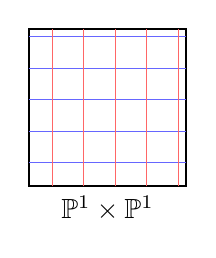
\begin{tikzpicture}[scale=2]
  % boundary square representing P^1 x P^1
  \draw[thick] (0,0) rectangle (1,1);

  % horizontal ruling (first P^1–factor)
  \foreach \y in {0.15,0.35,0.55,0.75,0.95}{
    \draw[blue!60] (0,\y) -- (1,\y);
  }

  % vertical ruling (second P^1–factor)
  \foreach \x in {0.15,0.35,0.55,0.75,0.95}{
    \draw[red!60] (\x,0) -- (\x,1);
  }

  % sample fiber labels
  % \node[blue!70!black, anchor=east] at (-0.02,0.75) {$\{p\}\times\mathbb{P}^1$};
  % \node[red!70!black, anchor=south] at (0.75,1.02) {$\mathbb{P}^1\times\{q\}$};

  % corner label
  \node[below] at (0.5,0) {$\mathbb{P}^1\times\mathbb{P}^1$};
\end{tikzpicture}
    % \caption{A 4-chain in $\mathbb{P}^3$.}
    \label{fig:Q_4}
    \end{figure}
\end{frame}

\begin{frame}{4-chain}
    \begin{theorem}
        A 4-chain can be included in a singular quadric surface $X$.
    \end{theorem}

    \begin{itemize}
        \item Pair the lines as $(l_1, l_2)$ and $(l_3, l_4)$.
        \item $(l_1, l_2)$ can be included in a plane $H_1$.
        \item $(l_3, l_4)$ can be included in a plane $H_2$.
        \item Then $X = H_1 \cup H_2$ is a singular quadric surface including $Q_4$.
    \end{itemize}

    Include a figure of two planes including a 4-chain.
\end{frame}

\begin{frame}{6-chain}
    \begin{theorem}
        A regular 6-chain is included in a unique cubic surface
        $X$, which is singular.
    \end{theorem}
\end{frame}

\begin{frame}
    Singular surface as in 4-chain.
    Include figure.
\end{frame}

\begin{frame}
    \begin{theorem}
        In a smooth cubic surface, one can find at most a regular 5-chain.
    \end{theorem}
\end{frame}

\begin{frame}
    If one smooth surface, then many.
\end{frame}

\begin{frame}
    Uniqueness.
\end{frame}

\end{document}